\documentclass[border=6pt]{standalone}
\usepackage[T1]{fontenc}
\usepackage{amsmath, amssymb}
\usepackage{tikz}
\usetikzlibrary{shapes.multipart}

% --------------------------------------------------- Farben
\definecolor{physfill}{HTML}{DCE9F5}
\definecolor{physline}{HTML}{2C5F8A}

\newcommand{\cd}[1]{\texttt{#1}}

\begin{document}
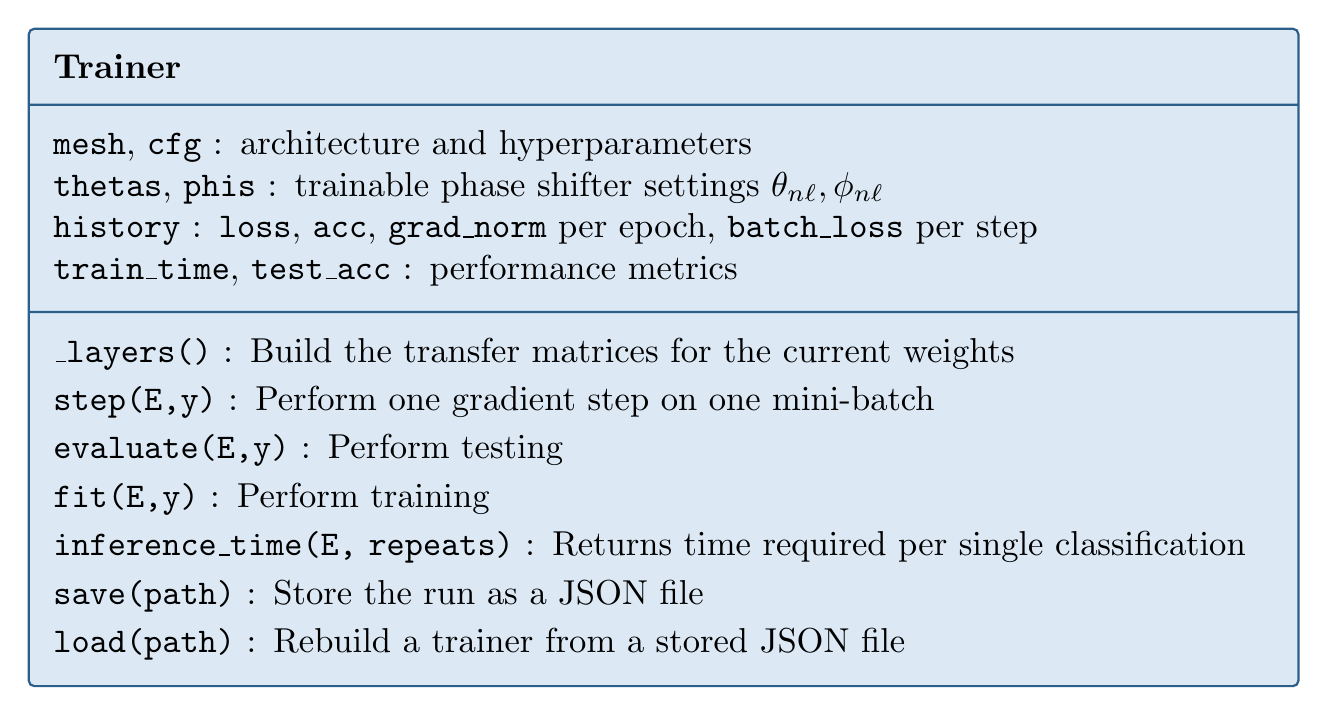
\begin{tikzpicture}[
    scale=1.25, transform shape,
    font=\normalsize,
    cls/.style   = {rectangle split, rectangle split parts=3,
                    rectangle split part align=left,
                    draw, thick, rounded corners=2pt,
                    fill=physfill, draw=physline,
                    text width=124mm, align=left, inner sep=2.5mm}
  ]

% =========================================================================
%  Das Klassendiagramm
% =========================================================================
\node[cls] (tr)
  {\textbf{Trainer}
   \nodepart{two}
   \cd{mesh}, \cd{cfg} : architecture and hyperparameters\\
   \cd{thetas}, \cd{phis} : trainable phase shifter settings
     $\theta_{n\ell},\phi_{n\ell}$\\
   \cd{history} : \cd{loss}, \cd{acc}, \cd{grad\_norm} per epoch,
     \cd{batch\_loss} per step\\
   \cd{train\_time}, \cd{test\_acc} : performance metrics
   \nodepart{three}
   \cd{\_layers()} : Build the transfer matrices for the current weights
   %$\rightarrow\ [\hat{M}_j]$ for the current phases
     %-- rebuilt after every update
     \\[0.7mm]
   \cd{step(E,y)} : Perform one gradient step on one mini-batch
   %-- one minibatch: forward $\rightarrow\ \Gamma_L\
     %\rightarrow$ adjoint $\rightarrow\ \nabla\ \rightarrow$ update\\
   %\quad returns $(\mathcal{L},\,\lVert\nabla\rVert_2)$
   \\[0.7mm]
   \cd{evaluate(E,y)} : Perform testing
   %$\rightarrow\ (\mathcal{L},\text{accuracy})$,
     %leaves the phases unchanged
     \\[0.7mm]
   \cd{fit(E,y)} : Perform training
   %-- epochs $\times$ minibatches, stops on
     %\cd{patience} / \cd{max\_epochs},\\
   %\quad keeps the best phases
   \\[0.7mm]
   \cd{inference\_time(E, repeats)} : Returns time required per single classification
   % -- seconds per classification
     %(matrices excluded)
     \\[0.7mm]
    \cd{save(path)} : Store the run as a JSON file
    \\[0.7mm]
     \cd{load(path)} : Rebuild a trainer from a stored JSON file
     };
\end{tikzpicture}
\end{document}